\section{3D Geometry}
\label{sec:3d_geometry}

\begin{frame}
    \frametitle{3D coordinates}
    \begin{figure}
        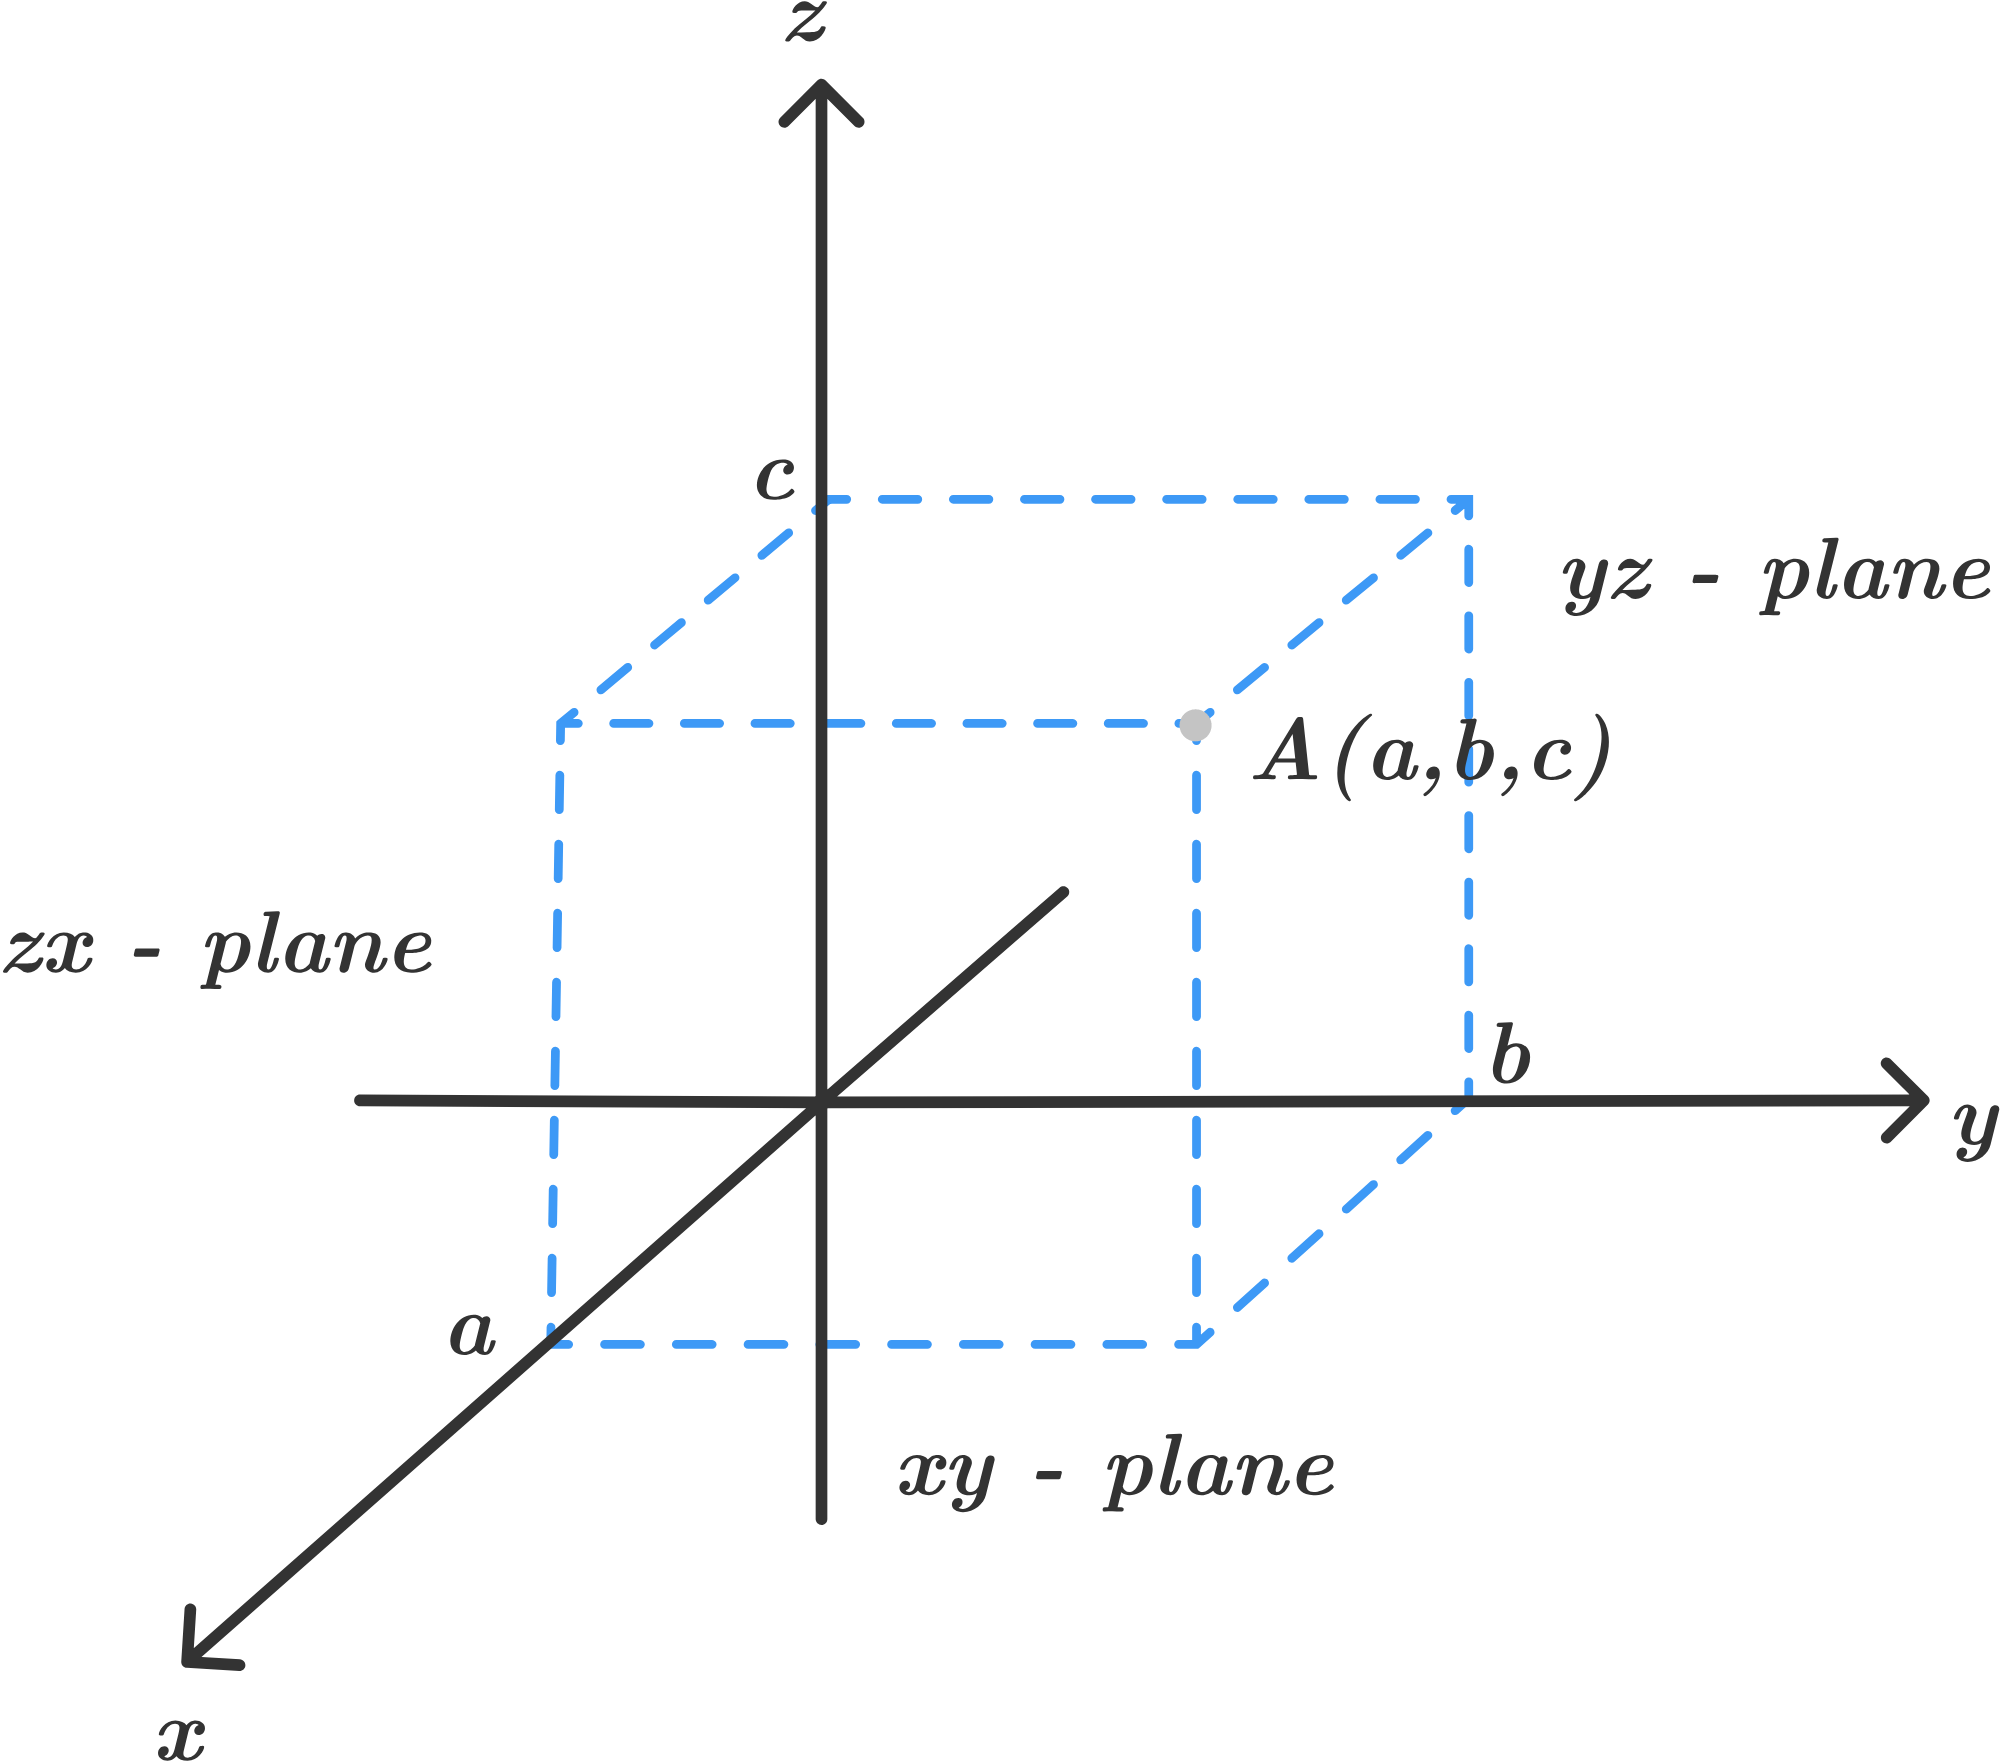
\includegraphics[scale=0.1]{3d_geometry/co_ordinate_plane.png}
        \caption{3D Coordinate Plane}
    \end{figure}
\end{frame}

\begin{frame}
    \frametitle{3D Coordinate System}
    \begin{itemize}
        \item The 3D coordinate system is defined by three mutually perpendicular axes: the x-axis, y-axis, and z-axis.
        \item A point in 3D space is represented by its coordinates \(P(x, y, z)\).
        \item The position vector of a point \(P\) in 3D space is given by:
        \[
        \vec{OP} = x\hat{\imath} + y\hat{\jmath} + z\hat{k}
        \]
    \end{itemize}       
\end{frame}

\begin{frame}
    \frametitle{Shifting the Origin}
    \begin{block}{Translation of Axes}
        Shifting the origin  to another point without changing the direction of axes is called \textbf{translation}.
    \end{block}
   Let the origin \(O\) be shifted to a new point \(O'\) with coordinates \(O'(x_0, y_0, z_0)\). The position vector of a point \(P(x,y,z)\) with respect to the new origin \(O'\) given by :
    \[
        \vec{O'P} = (x - x_0)\hat{\imath} + (y - y_0)\hat{\jmath} + (z - z_0)\hat{k}
    \]
\end{frame}

\begin{frame}
\frametitle{Distance Formula in 3D}
\begin{figure}
    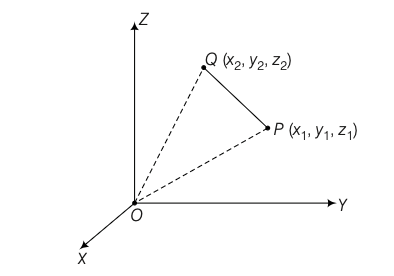
\includegraphics[scale=0.1]{3d_geometry/distance.png}
    \caption{Distance Formula in 3D}
\end{figure}
Let \(OP = x \hat{\imath} + y \hat{\jmath} + z \hat{k}\)  and \(OQ = x' \hat{\imath} + y' \hat{\jmath} + z' \hat{k}\) be two points in 3D space. The distance \(d\) between points \(P\) and \(Q\) is given by the formula:
\begin{align*}
    \vec{OQ} &= \vec{OP} + \vec{PQ} \\
    \vec{PQ} &= \vec{OQ} - \vec{OP} \\
    d &= |\vec{PQ}| = \sqrt{(x' - x)^2 + (y' - y)^2 + (z' - z)^2}
\end{align*}
\end{frame}

\begin{frame}
    \frametitle{Section Formula}
    \begin{figure}
        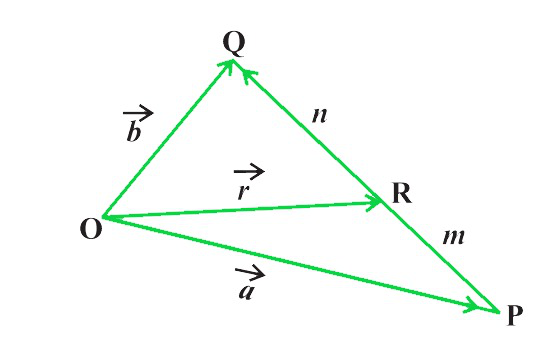
\includegraphics[scale=0.3]{3d_geometry/section.png}
        \caption{Section Formula in 2D}
    \end{figure} 
\end{frame}


\begin{frame}
    \begin{block}{Section Formula in 3D}
    Let \(P(x_1, y_1, z_1)\) and \(Q(x_2, y_2, z_2)\) be two points in 3D space with position vectors \( \vec{\mathbf{r}_1} \), \( \vec{\mathbf{r}_2} \) respectively. If a point \(R\) divides the line segment \(PQ\) in the ratio \(m:n\), then the position vector of point \(R\) is given by:
    \[
    \vec{\mathbf{r}} = \frac{m\vec{\mathbf{r}_2} + n\vec{\mathbf{r}_1}}{m+n}
    \]
    \end{block}
\end{frame}

\begin{frame}
    \frametitle{Proof of Section Formula}
    \begin{block}{Given}
    Point \(R\) divides line segment \(PQ\) internally in the ratio \(m:n\), where \(P\) and \(Q\) have position vectors \(\vec{\mathbf{r}_1}\) and \(\vec{\mathbf{r}_2}\) respectively.
    \end{block}
    
    \begin{block}{To Prove}
    The position vector of \(R\) is \(\vec{\mathbf{r}} = \frac{m\vec{\mathbf{r}_2} + n\vec{\mathbf{r}_1}}{m+n}\)
    \end{block}
    
    \begin{block}{Proof}
    Since \(R\) divides \(PQ\) in ratio \(m:n\):
    \begin{align}
        \frac{|\vec{PR}|}{|\vec{RQ}|} &= \frac{m}{n} \\
        \text{Since } \vec{PR} \text{ and } \vec{RQ} \text{ are collinear:} \quad \vec{PR} &= \frac{m}{n}\vec{RQ}
    \end{align}
    \end{block}
\end{frame}

\begin{frame}
    \frametitle{Proof of Section Formula (continued)}
    \begin{block}{Proof (continued)}
    From vector addition: \(\vec{PR} + \vec{RQ} = \vec{PQ}\)
    
    Substituting \(\vec{PR} = \frac{m}{n}\vec{RQ}\):
    \begin{align}
        \frac{m}{n}\vec{RQ} + \vec{RQ} &= \vec{PQ} \\
        \vec{RQ}\left(\frac{m}{n} + 1\right) &= \vec{PQ} \\
        \vec{RQ} &= \frac{n}{m+n}\vec{PQ}
    \end{align}
    
    Since \(\vec{PQ} = \vec{\mathbf{r}_2} - \vec{\mathbf{r}_1}\) and \(\vec{RQ} = \vec{\mathbf{r}_2} - \vec{\mathbf{r}}\):
    \begin{align}
        \vec{\mathbf{r}_2} - \vec{\mathbf{r}} &= \frac{n}{m+n}(\vec{\mathbf{r}_2} - \vec{\mathbf{r}_1}) \\
        \vec{\mathbf{r}} &= \vec{\mathbf{r}_2} - \frac{n}{m+n}(\vec{\mathbf{r}_2} - \vec{\mathbf{r}_1}) \\
        \vec{\mathbf{r}} &= \frac{m\vec{\mathbf{r}_2} + n\vec{\mathbf{r}_1}}{m+n}
    \end{align}
    \end{block}
\end{frame}



